\documentclass[twoside]{scrartcl}
\usepackage[utf8]{inputenc}
\usepackage[T1]{fontenc}
\usepackage{lmodern}
\usepackage{latexsym}
\usepackage{amsfonts}
\usepackage{amssymb}
\usepackage{fancyhdr,lastpage}
\usepackage{hyperref}
\usepackage{graphicx}
\usepackage{wrapfig}
\usepackage{amsmath}
\usepackage{geometry}
\usepackage[ngerman]{babel}
\geometry{hmargin={2cm,2cm},vmargin={2.4cm,3cm}}
\usepackage{comment}
\newcommand{\llfloor}{\left\lfloor}
\newcommand{\rrfloor}{\right\rfloor}
\setlength{\headheight}{20pt}
\pagestyle{fancy}
\fancyhf{}
\fancyhead[L]{Algorithm Proposal}
\fancyhead[C]{Fabian Hirschmann, Michael Markert}
\fancyhead[R]{\today}
\fancyfoot[C]{Page \thepage\ of \pageref{LastPage}}
\begin{document}
\section{Definition}
Die \texttt{Qualität} eines Algorithmus zur Streckengeneralisierung
wird durch den Abstand von der ursprünglichen Streckenführung
beschrieben.\\\\
Mit zunehmender Reduzierung der Stützpunkte einer Streckenführung
nimmt die Qualität der generalisierten Streckenführung für
gewöhnlich ab.
\section{Vorauswahl}
Bahnhöfe werden in einen Status versetzt, in dem sie von keinen
Algorithmus aus der Streckenführung entfernt werden können.
\section{Kombination}
\subsection{Algorithmus 1}
Die Stützpunkte zweier Streckenführungen
$s_1, s_2 \in \{(x_0, y_0), (x_1, y_1), \ldots, (x_n, y_n)\}$
werden angeglichen indem die Stützpunkte
$a \in s_1$ und  $b \in s_2$ $a = b$ gesetzt wird, falls
$|a - b| < \varepsilon$ gilt.\\
\\
Dies dient hauptsächlich dazu, dass nahe beieinander liegende
Streckenverläufe nach Anwendungen weiterer Algorithmen auch
wieder beieinander liegen.
\subsection{Algorithmus 2}
Die Karte wird in ein Raster eingeteilt. Alle Stützpunkte innerhalb
Rasterzelle werden zusammengefasst.
\section{Vereinfachung}
\subsection{Algorithmus 1: Ramer-Douglas-Peucker Algorithmus}
Durch die Anwendung des Ramer-Douglas-Pleucker Algorithmus
(Abbildung 1) 
wird durch Reduzierung der Stützpunkte eine Vereinfachung
der Streckenführung erreicht.\\

\begin{wrapfigure}{r}{0.5\textwidth}
  \begin{center}
    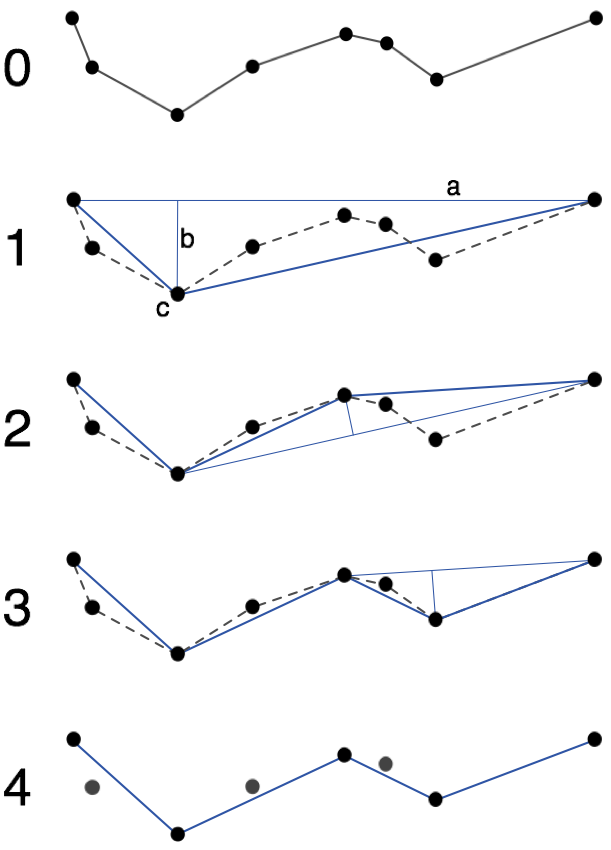
\includegraphics[scale=0.20]{rdp.png}
  \end{center}
  \caption{R-D-P Visualisierung}
\end{wrapfigure}

Abbildung 1 zeigt die Visualisierung des Ramder-Douglas-Peucker
Algorithmus.\\
Als Start- und Endpunkte werden Bahnhöfe gewählt. Auf die daraus
resultierenden Streckenabschnitte wird der R-D-P Algorithmus
angewendet.

\end{document}
